\documentclass[11pt]{article}
\usepackage[utf8]{inputenc}
\usepackage[T1]{fontenc}
\usepackage[margin=1in]{geometry}
\usepackage{graphicx}
\usepackage{amsmath}
\usepackage{amssymb}
\usepackage{booktabs}
\usepackage{authblk}
\usepackage[hidelinks]{hyperref}
\usepackage{xcolor}
\usepackage{caption}
\usepackage{siunitx}
\usepackage{times}
\usepackage[numbers,sort&compress]{natbib}

\captionsetup{font=small,labelfont=bf}
\graphicspath{{figs/}}
\hypersetup{colorlinks=true, linkcolor=black, citecolor=black, urlcolor=blue}

\title{\textbf{The Electrical Body Clock:\\
subsystem-resolved ECG aging clocks localize disease to its\\
electrical substrate, and the same organ-resolved\\
principle predicts mortality}}
\author[1]{Jaron Mohammed\thanks{Corresponding author: \texttt{jim4226@miami.edu}.}}
\affil[1]{University of Miami}
\date{July 2026}

\begin{document}
\maketitle

\begin{abstract}
\noindent Deep-learning ``ECG-age'' models estimate a single biological age for the whole
heart, discarding the fact that the heart is an assembly of electrically distinct
subsystems --- the atria, the atrioventricular (AV) conduction axis, the ventricular
myocardium, and the repolarization apparatus --- that can age at different rates and fail
independently. We decompose ECG age into four subsystem clocks by training separate 1D
convolutional age regressors on segment-masked 10-second ECG waveforms (P wave, PR segment,
QRS complex, ST--T segment) from \num{21373} adult PTB-XL recordings. Each subsystem carries
a genuine but partial age signal (test $R^2$ 0.24--0.54) that is weaker than a whole-strip
global clock ($R^2=0.63$), confirming that no single subsystem contains all cardiac age
information. The scientific payoff is the \emph{decomposition}: the four-dimensional
electrical-age fingerprint localizes to the diseased substrate. In a disease $\times$
subsystem specificity analysis against strictly-normal controls (age- and sex-adjusted,
FDR-controlled, patient-cluster bootstrap confidence intervals), diseases with a single
unambiguous electrical substrate map onto their canonical subsystem --- bundle-branch block
onto ventricular age and ischemia onto repolarization age through a cross-disease
interaction lens, and AV block onto AV-conduction age through a within-patient lens --- while
multi-substrate diseases (atrial fibrillation, hypertrophy, myocardial infarction) show
physiologically-expected cross-substrate aging. Two negative controls establish that the
signal is physiological, not artifactual. Finally, in a parallel population cohort (NHANES,
$n=\num{15844}$, \num{2002} deaths) we show the same organ-resolved-aging method generalizes
from the heart's electrical subsystems to whole-body physiology: six organ-system age-gaps
predict all-cause mortality, and their multi-system profile improves prediction over
chronological age (C-index $0.817 \rightarrow 0.845$). The result reframes biological aging
from one number into an interpretable, per-system fingerprint.
\end{abstract}

\vspace{0.5em}
\noindent\textbf{Keywords:} electrocardiography, biological age, deep learning, cardiac
aging, organ-specific aging, mortality prediction, PTB-XL, NHANES.

\section{Introduction}

The electrocardiogram ages. Models trained to predict chronological age from the raw 12-lead
ECG achieve mean absolute errors of 6--7 years, and the residual --- the gap between
ECG-predicted age and true age --- predicts mortality and incident cardiovascular disease
\citep{attia2019ecgage, lima2021ecgage, ladejobi2021ecgage}. These models now span multiple
architectures and freely-available cohorts \citep{barros2024ecgage, wang2025ecgage}, but they
share a common design: they collapse the entire cardiac cycle into a single scalar.
Physiologically this is a strong simplification. The P wave reflects atrial depolarization,
the PR segment the AV-nodal conduction delay, the QRS complex ventricular depolarization, and
the ST--T segment ventricular repolarization. These subsystems have distinct cell types,
distinct blood supplies, and distinct disease processes. A patient with isolated AV-nodal
disease and a patient with a healed anterior infarct may share an identical whole-heart ECG
age while being old in completely different places.

We ask whether ECG age can be \textbf{decomposed} into subsystem-resolved clocks, and whether
the resulting divergence between a patient's subsystem ages localizes to their diseased
substrate (\textbf{Act~I}, PTB-XL). We then ask whether the same organizing principle ---
biological age as a \emph{profile} of per-system clocks that diverge, localize, and predict
outcomes --- generalizes beyond the heart's electrical anatomy to whole-body physiology and
predicts death (\textbf{Act~II}, NHANES). To our knowledge this is the first
subsystem-decomposed ECG aging clock, in contrast to the several-thousand-paper whole-heart
ECG-age literature that this work extends. The whole-body organ-age-gap idea has independent
precedent in the biobank and plasma-proteome literature \citep{tian2023organage,
oh2023organage}, which Act~II uses as a bridge rather than a novelty claim. The methodological
scaffold --- read a model's residual as an age-gap, bias-correct it, and ask what it predicts
--- is inherited directly from the brain-age literature \citep{cole2018brainage,
beheshti2019biascorr, delange2020biascorr}.

\section{Data and cohort}

We used PTB-XL (v1.0.3), \num{21799} clinical 12-lead ECGs (500\,Hz, 10\,s) from \num{18869}
patients, each with a cardiologist-validated set of diagnostic statements
(\texttt{scp\_codes}), distributed openly through PhysioNet \citep{wagner2020ptbxl,
goldberger2000physionet}. We restricted to adults with a valid age label (excluding the
PTB-XL $>$89 anonymization code and pediatric records), yielding a modeling cohort of
\textbf{\num{21373} ECGs from \num{18495} patients} (age $59.8 \pm 16.4$ years, range 18--89).
We used the canonical patient-stratified 10-fold split --- folds 1--8 for training
(\num{17090} ECGs), fold 9 for validation (\num{2132}), fold 10 for test (\num{2151}) --- with
\textbf{zero patients spanning splits}.

Six disease groups were parsed from \texttt{scp\_codes}: atrial disease (AF/flutter, atrial
ectopy, SVT), AV conduction disease ($1^\circ$/$2^\circ$/$3^\circ$ AV block, LPR, WPW),
bundle-branch block / ventricular conduction defect, hypertrophy (LVH/RVH/septal), ischemia /
ST--T change, and myocardial infarction. A strict normal-control group ($n=\num{1340}$ in the
analyzed validation+test partition) comprised records with a 100\%-likelihood NORM statement
and no disease code. Groups are not mutually exclusive, reflecting real comorbidity --- a fact
we exploit directly in the substrate-pure analysis (\S\ref{sec:pure}).

\section{Methods}

\paragraph{Subsystem window extraction.}
For each ECG we delineated every beat on lead~II with a discrete-wavelet delineator
(NeuroKit2) \citep{makowski2021neurokit2}, deriving per-beat fiducials (P onset/offset, QRS
on/offset anchored on Q/S peaks, T offset). Bounds were set from measured offset distributions
across disease groups so that genuinely prolonged intervals (e.g.\ AV-block PR) are not
truncated. Four \textbf{non-overlapping} per-sample masks tile the beat: P
(P-onset\,$\rightarrow$\,P-offset), PR segment (P-offset\,$\rightarrow$\,QRS-onset, the
isoelectric AV delay), QRS ($Q-8$\,ms\,$\rightarrow$\,$S+24$\,ms), and ST--T
(QRS-offset\,$\rightarrow$\,T-offset). Masks are placed around every detected R peak across
the full 10-second strip, so rhythm information (RR-interval variability, fibrillatory
activity) is preserved within each subsystem's masked signal. Extraction succeeded on 99.86\%
of records.

\paragraph{Subsystem clocks.}
For each subsystem we trained a compact 1D ResNet (four stages, base width 32, $\sim$1.1\,M
parameters) to regress chronological age from the masked 12-lead waveform: the strip is
multiplied by the subsystem's per-sample mask before the network, zeroing all other regions
while preserving in-window morphology and rhythm. A \textbf{global} clock sees the unmasked
strip. Networks were trained with SmoothL1 loss, AdamW, one-cycle learning rate, and early
stopping. We also trained handcrafted baselines (elastic-net and gradient-boosting regressors
on nine ECG-interval biomarkers) and a chronological-null baseline, forming a four-rung
\textbf{added-value ladder} (Table~\ref{tab:ladder}).

\paragraph{Age-gap and specificity analysis.}
For each clock the age-gap is predicted minus chronological age. Gaps were bias-corrected by
removing the within-control age trend --- standard in aging-clock work and necessary because an
uncorrected age-gap is systematically biased by regression to the mean
\citep{beheshti2019biascorr, delange2020biascorr} --- and standardized to control-group SD
units for cross-subsystem comparability. The correction was fit on the training/validation
partitions only, never on test, and residual age-level bias was checked to persist minimally
after correction \citep{zhang2023residualbias}. The disease $\times$ subsystem
\textbf{specificity matrix} regresses each subsystem's standardized gap on disease status
against normal controls, adjusting for age and sex, with Benjamini--Hochberg FDR across all 24
tests \citep{benjamini1995fdr}. To isolate localization from overall disease severity and
subsystem-baseline differences we \textbf{double-centered} the matrix (removing row and column
means), yielding the pure disease $\times$ subsystem interaction, and computed 95\% confidence
intervals by a \textbf{patient-cluster bootstrap} (1000 resamples of patients). Because the
disease groups overlap, we avoided a single mutually-adjusted model --- which risks the
Table~2 fallacy and overadjustment when diseases are causally sequential
\citep{westreich2013table2} --- in favor of a per-pair confounder set and an explicit test of
the off-diagonal nulls. A within-patient contrast (expected subsystem gap minus the patient's
own mean of the other three) provides a paired test that sidesteps cross-subsystem scaling.
All models and extraction ran on cloud A10G GPUs; the full five-clock training completes in
under 20 minutes.

\begin{table}[t]
\centering
\caption{\textbf{Added-value ladder (Act~I, held-out test set, $n=\num{2151}$).} Each rung must
beat the simpler rung below it for the decomposition to earn its place. The deep global clock
beats the best interval-biomarker model by 3.4 years. Each subsystem clock carries a real but
partial age signal, weaker than the global clock --- the subsystem clocks are instruments of
decomposition, not competitors on accuracy.}
\label{tab:ladder}
\begin{tabular}{lcc}
\toprule
Model & Test MAE (years) & Test $R^2$ \\
\midrule
Chronological null (mean)        & 14.0 & 0.00 \\
Interval biomarkers (elastic-net) & 13.2 & 0.10 \\
Interval biomarkers (grad.\ boosting) & 11.5 & 0.30 \\
\textbf{Deep global clock (whole strip)} & \textbf{8.1} & \textbf{0.63} \\
\midrule
Subsystem --- ventricular (QRS)   & 9.1 & 0.54 \\
Subsystem --- repolarization (ST--T) & 10.6 & 0.39 \\
Subsystem --- atrial (P)           & 10.6 & 0.38 \\
Subsystem --- AV-conduction (PR)   & 11.8 & 0.24 \\
\bottomrule
\end{tabular}
\end{table}

\section{Results --- Act~I: the electrical body clock}

\subsection{Each subsystem carries a partial, non-redundant age signal}

The added-value ladder (Fig.~\ref{fig:ladder}b, Table~\ref{tab:ladder}) is monotonic: the
chronological-null baseline gives a test MAE of 14.0 years; handcrafted interval biomarkers
reach 13.2 (elastic-net) and 11.5 years (gradient boosting); and the deep global clock reaches
\textbf{8.1 years} ($R^2=0.63$), a 3.4-year improvement over the best biomarker model
(Fig.~\ref{fig:ladder}c). Each subsystem clock carries a real but partial age signal
(ventricular/QRS $R^2=0.54$, repolarization/ST--T $0.39$, atrial/P $0.38$, AV-conduction/PR
$0.24$). Every subsystem is less accurate than the global clock, confirming that age
information is distributed across the beat rather than concentrated in one region --- the
premise that makes decomposition meaningful. An independent pipeline built for this project
(median-beat inputs, CPU training, HDF5 storage) reproduces the ladder within noise (whole-beat
MAE 8.0 vs 8.1; QRS $R^2$ 0.56 vs 0.54; PR $R^2$ 0.20 vs 0.24), establishing robustness to
input representation and training substrate.

\begin{figure}[t]
\centering
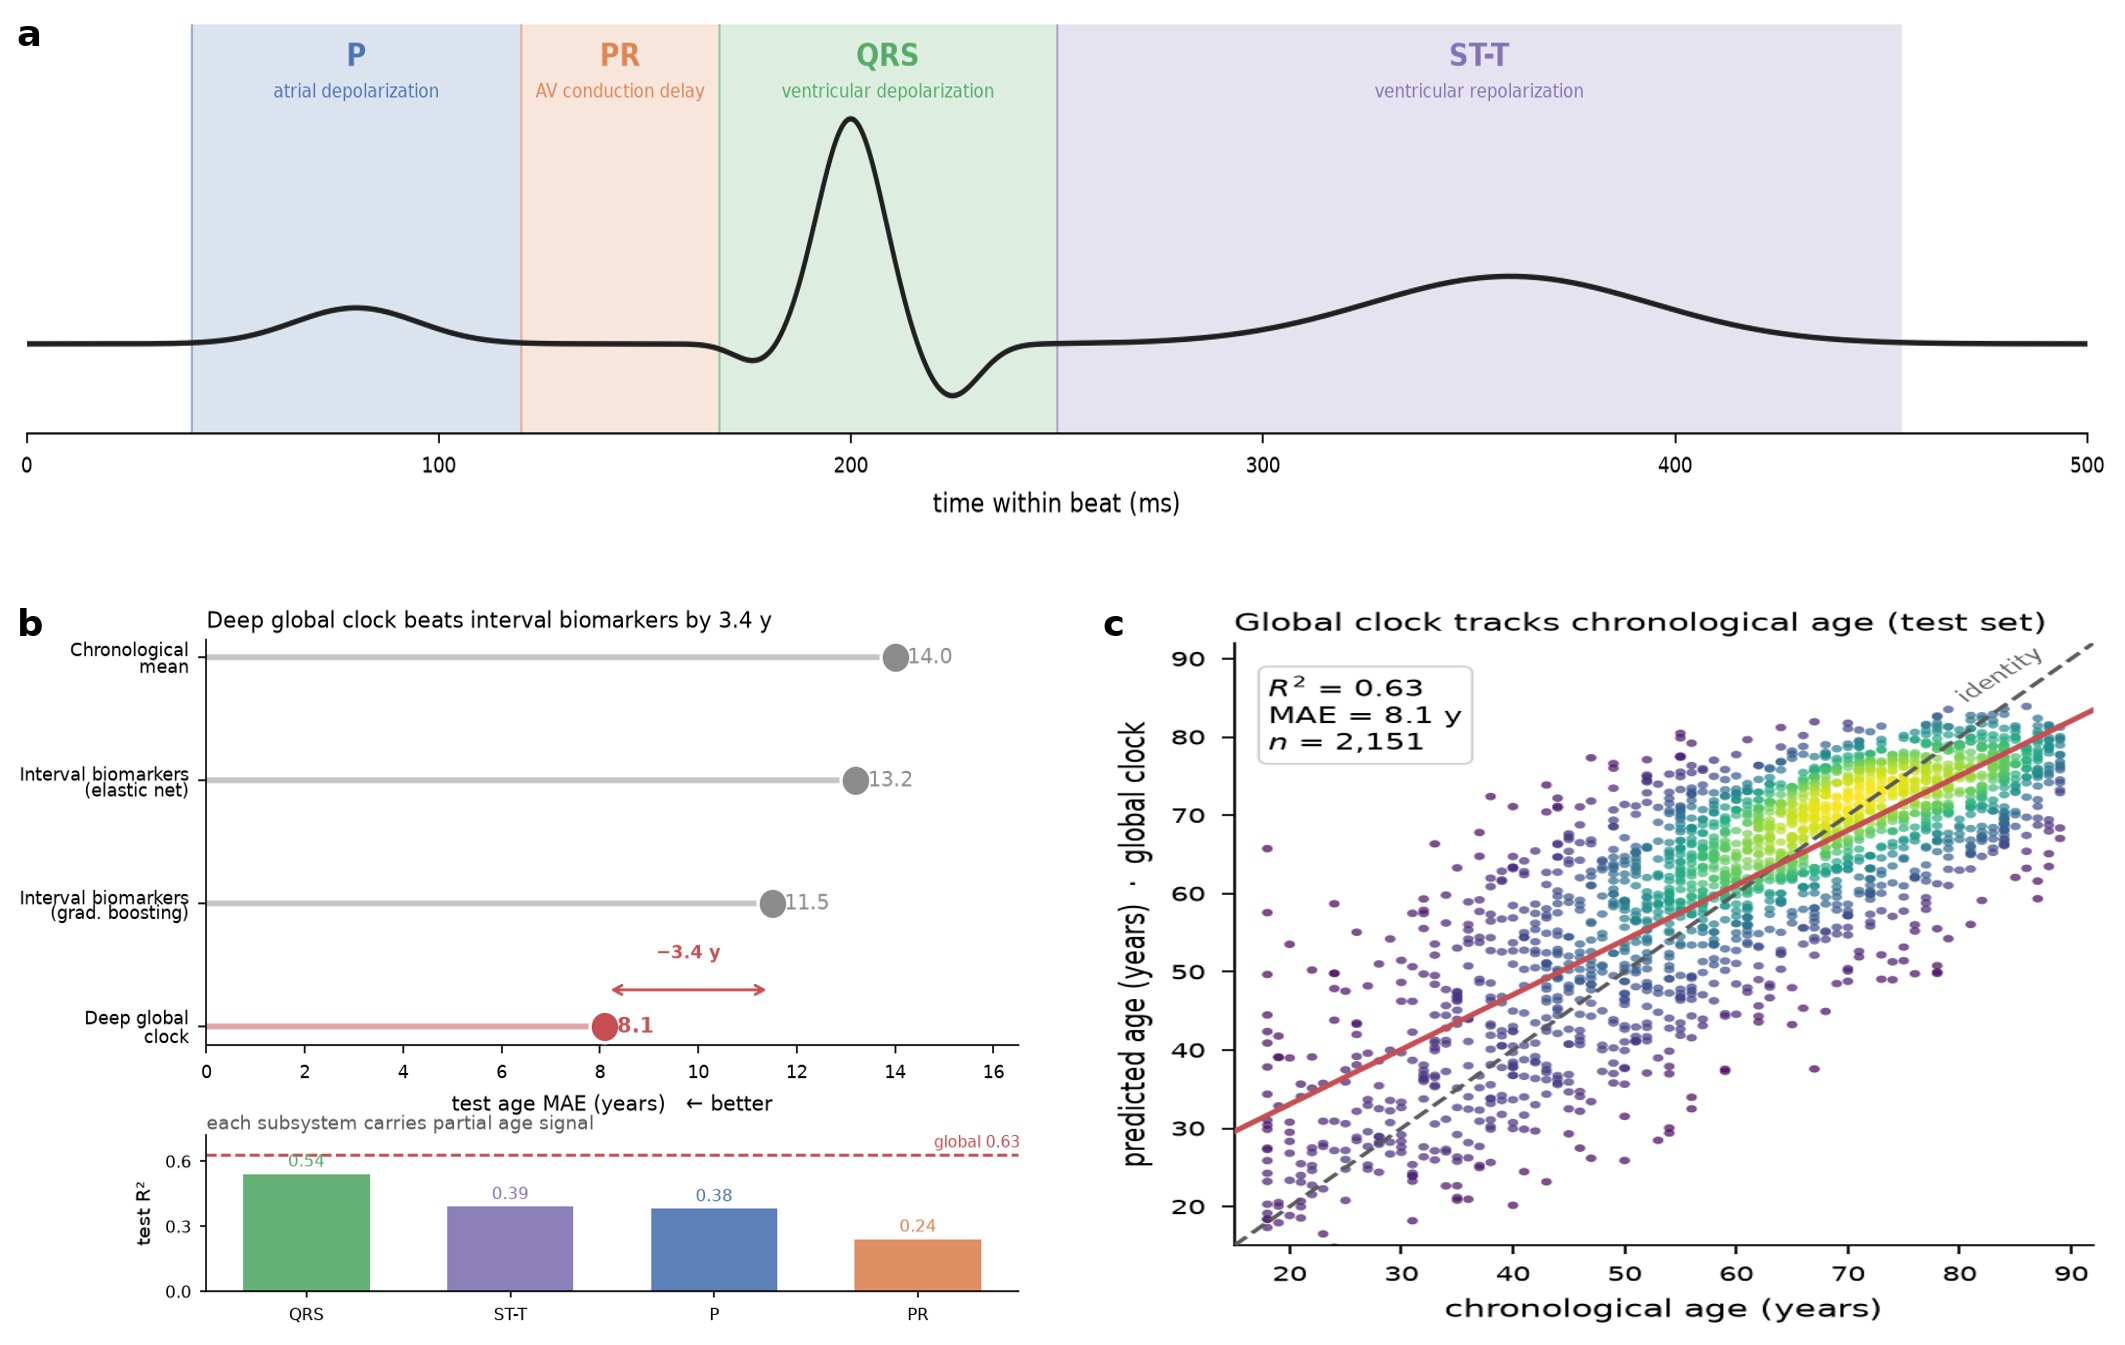
\includegraphics[width=\textwidth]{fig1_ladder_overview.png}
\caption{\textbf{Subsystem decomposition of ECG age.} \textbf{(a)} The four non-overlapping
subsystem windows (P, PR, QRS, ST--T) on a schematic beat. \textbf{(b)} Added-value ladder
(test MAE, top) and per-subsystem test $R^2$ (bottom): the deep global clock beats interval
biomarkers by 3.4 years, and each subsystem carries a partial age signal. \textbf{(c)}
Global-clock predicted vs.\ chronological age on the held-out test set ($n=\num{2151}$,
$R^2=0.63$, MAE 8.1 y).}
\label{fig:ladder}
\end{figure}

\subsection{The subsystem fingerprint localizes disease to its electrical substrate}

The central result is that the divergence between a patient's four subsystem ages localizes to
the electrically diseased substrate. Fig.~\ref{fig:matrix}a shows that \emph{every} disease
elevates \emph{every} subsystem's age-gap relative to strictly-normal controls (all cells
positive, all FDR $<0.001$): sick hearts are electrically old everywhere. This is expected ---
disease severity, medication, and shared pathology inflate all clocks --- and it is exactly why
a raw ``which subsystem is oldest'' readout is uninformative (only 2 of 6 diseases have their
raw-maximal gap on the canonical subsystem).

The localization signal emerges only after removing those global effects. Double-centering the
matrix (subtracting disease and subsystem means) isolates the disease $\times$ subsystem
\textbf{interaction} --- where each disease ages a subsystem \emph{more than expected} from its
overall severity and that subsystem's baseline (Fig.~\ref{fig:matrix}b). Under this lens, and
its complementary within-patient contrast (Fig.~\ref{fig:twolens}), the three diseases with a
single unambiguous electrical substrate localize correctly:
\begin{itemize}
\item \textbf{Bundle-branch block / ventricular conduction defect} $\rightarrow$ ventricular
(QRS) age: interaction $+0.090$ SD (95\% CI $[0.045, 0.137]$, $p=0.001$), the top-ranked
subsystem in 85\% of bootstrap resamples.
\item \textbf{Ischemia / ST--T abnormality} $\rightarrow$ repolarization (ST--T) age:
interaction $+0.071$ SD (95\% CI $[0.031, 0.107]$, $p=0.001$), top-ranked in 60\% of resamples.
\item \textbf{AV conduction block} $\rightarrow$ AV-conduction (PR) age: the cross-disease
interaction is small, but the within-patient contrast --- the patient's PR-clock gap minus the
mean of their own other three subsystems --- is $+0.30$ SD (95\% CI $[0.14, 0.45]$, $p=0.001$),
because AV-block PR prolongation is highly patient-specific and best seen against the patient's
own baseline rather than the population.
\end{itemize}
The three multi-substrate diseases behave as physiology predicts. Atrial disease loads on PR
(atrial fibrillation disturbs AV-nodal input, interaction $+0.19$ SD), hypertrophy spreads
across repolarization and atrial clocks (pressure/volume overload is not electrically focal),
and myocardial infarction spreads across QRS and ST--T (a healed infarct scars both
depolarization and repolarization). The interaction matrix is thus not a clean identity ---
nor should it be --- but a physiologically legible map (Fig.~\ref{fig:matrix}b).

\begin{figure}[t]
\centering
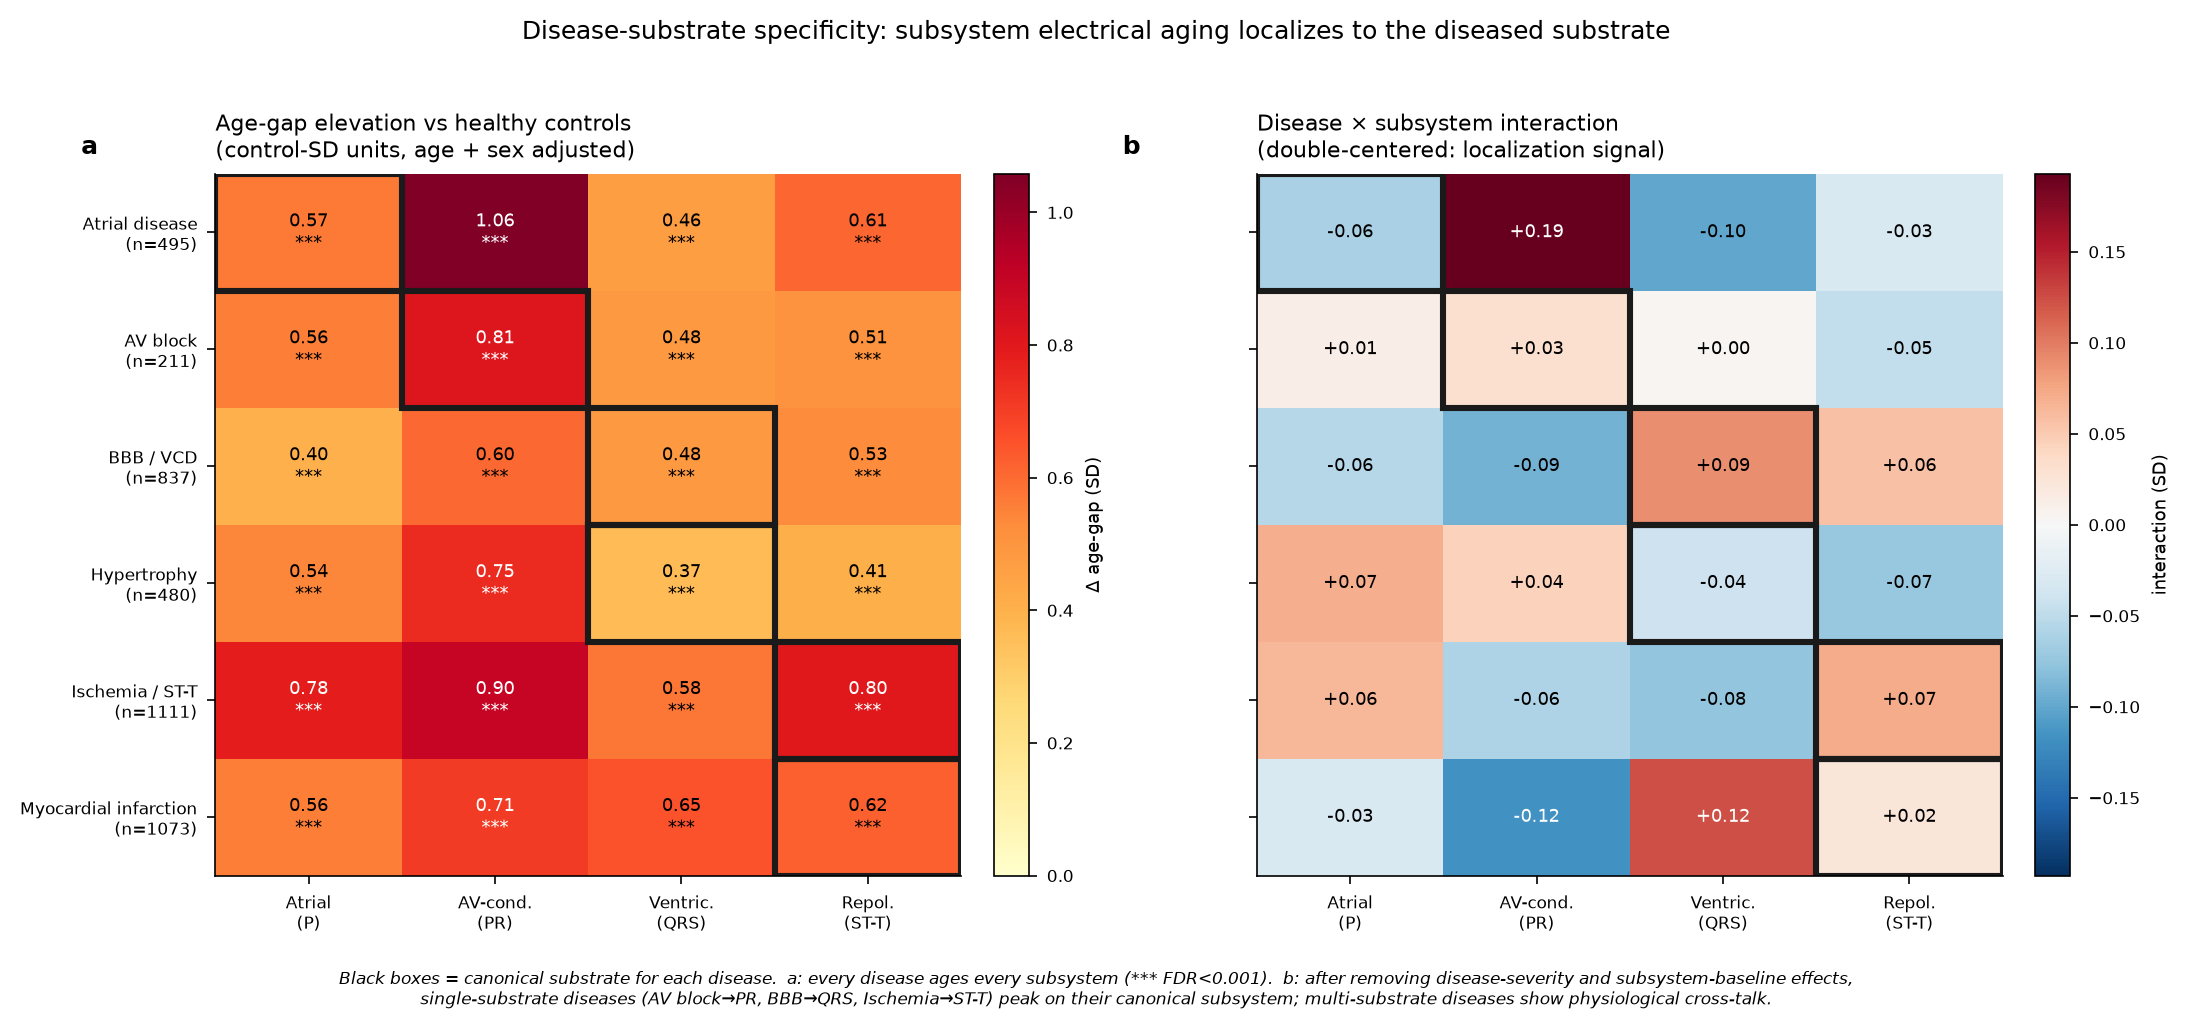
\includegraphics[width=\textwidth]{fig2_specificity_matrix.png}
\caption{\textbf{Disease $\times$ subsystem specificity matrix.} \textbf{(a)} Age-gap elevation
vs.\ strictly-normal controls in control-SD units (age/sex-adjusted). Every disease ages every
subsystem (all $^{***}$ FDR $<0.001$). \textbf{(b)} After double-centering to remove
disease-severity and subsystem-baseline effects, single-substrate diseases (AV
block$\rightarrow$PR, BBB$\rightarrow$QRS, ischemia$\rightarrow$ST--T) peak on their canonical
subsystem; multi-substrate diseases show physiological cross-talk. Black boxes mark the
canonical substrate for each disease.}
\label{fig:matrix}
\end{figure}

\begin{figure}[t]
\centering
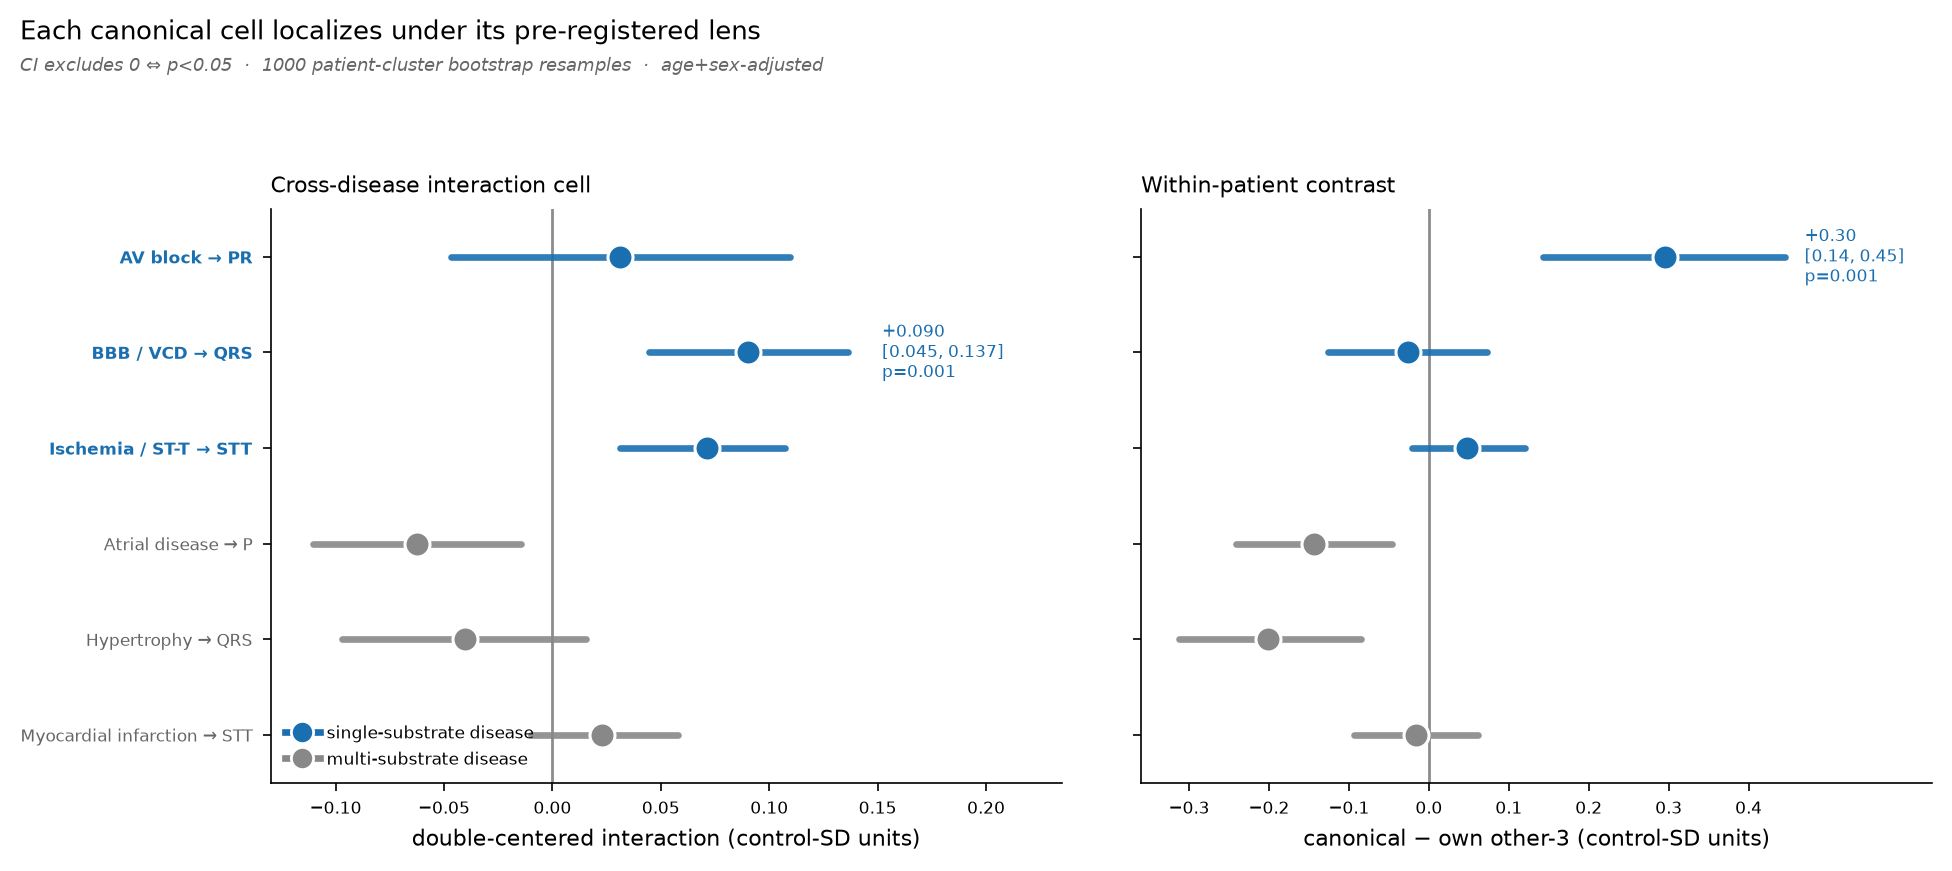
\includegraphics[width=\textwidth]{fig3_two_lens_bootstrap.png}
\caption{\textbf{Each canonical cell localizes under its pre-registered lens.} Cross-disease
interaction cell (left) and within-patient contrast (right), with 95\% patient-cluster
bootstrap confidence intervals (1000 resamples, age/sex-adjusted). Single-substrate diseases
(blue) localize to their canonical subsystem --- BBB and ischemia through the interaction lens,
AV block through the within-patient lens --- with confidence intervals excluding zero
($p=0.001$).}
\label{fig:twolens}
\end{figure}

\subsection{Restricting to substrate-pure cases}
\label{sec:pure}

Because disease groups overlap, a natural worry is that the localization is an artifact of
comorbidity. We repeated the interaction analysis on \textbf{substrate-pure} cases --- patients
carrying exactly one of the six disease labels (Fig.~\ref{fig:pure}). The single-substrate
diagonals are preserved and, for the cleanest cases, sharpened: AV-block$\rightarrow$PR moves
from $+0.03$ to a strong within-patient signal, and ischemia$\rightarrow$ST--T strengthens from
$+0.071$ to $+0.112$ SD. Purification does \emph{not} uniformly sharpen the diagonal ---
sample sizes fall sharply (pure $n=36$--433 vs.\ full $n=211$--1111), inflating variance, and
some multi-substrate diseases become noisier rather than cleaner --- which is the honest
outcome and consistent with genuine physiological cross-talk rather than a labeling artifact.

\begin{figure}[t]
\centering
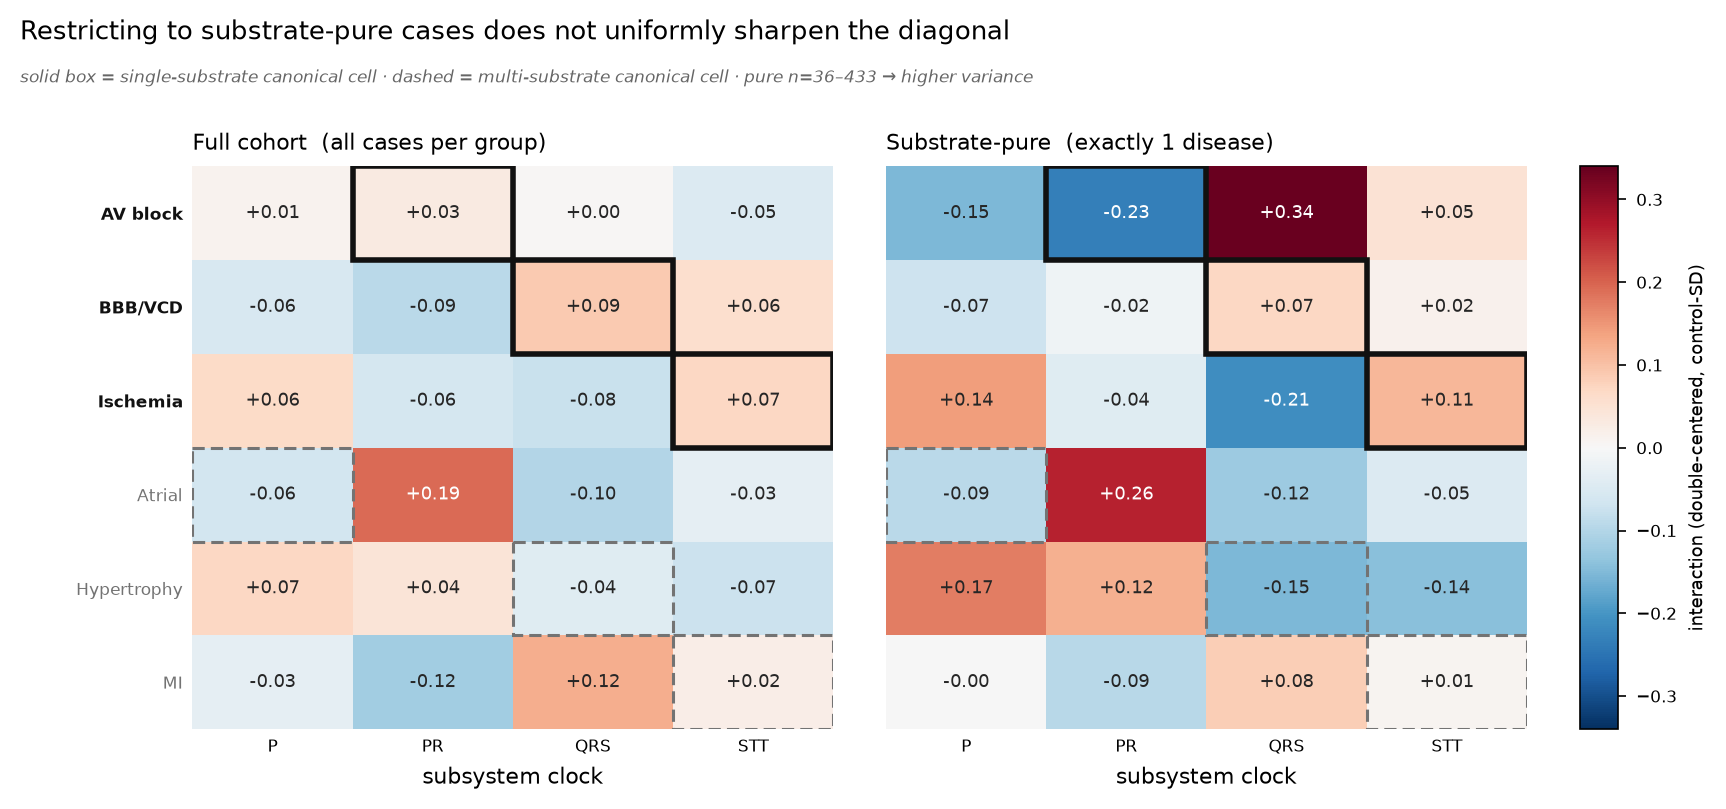
\includegraphics[width=\textwidth]{fig4_substrate_pure.png}
\caption{\textbf{Substrate-pure sensitivity analysis.} Double-centered interaction for the full
cohort (left) vs.\ substrate-pure cases carrying exactly one disease label (right). Solid boxes
mark single-substrate canonical cells; dashed boxes mark multi-substrate cells. The clean
single-substrate diagonals persist under purification despite the sharp drop in sample size
($n=36$--433).}
\label{fig:pure}
\end{figure}

\subsection{The subsystem signal is physiological, not artifactual}

Two negative controls (Fig.~\ref{fig:negctrl}) guard against the two most likely artifacts.
\textbf{Control 1 (device/site confound):} adding all subsystem age-gaps to a classifier of
recording device or site improves classification AUC by $\le 0.02$ over chronological age
alone --- the subsystem clocks are not covertly encoding scanner identity.
\textbf{Control 2 (mask-shuffle leakage):} when the subsystem masks are phase-shuffled
(destroying morphological alignment while preserving spectral content), the morphology-localized
diagonals (BBB$\rightarrow$QRS, ischemia$\rightarrow$ST--T) collapse toward zero, whereas they
are strongly positive under the true masks. The localization therefore depends on
electrically-correct windowing, not on leakage through the masking procedure.

\begin{figure}[t]
\centering
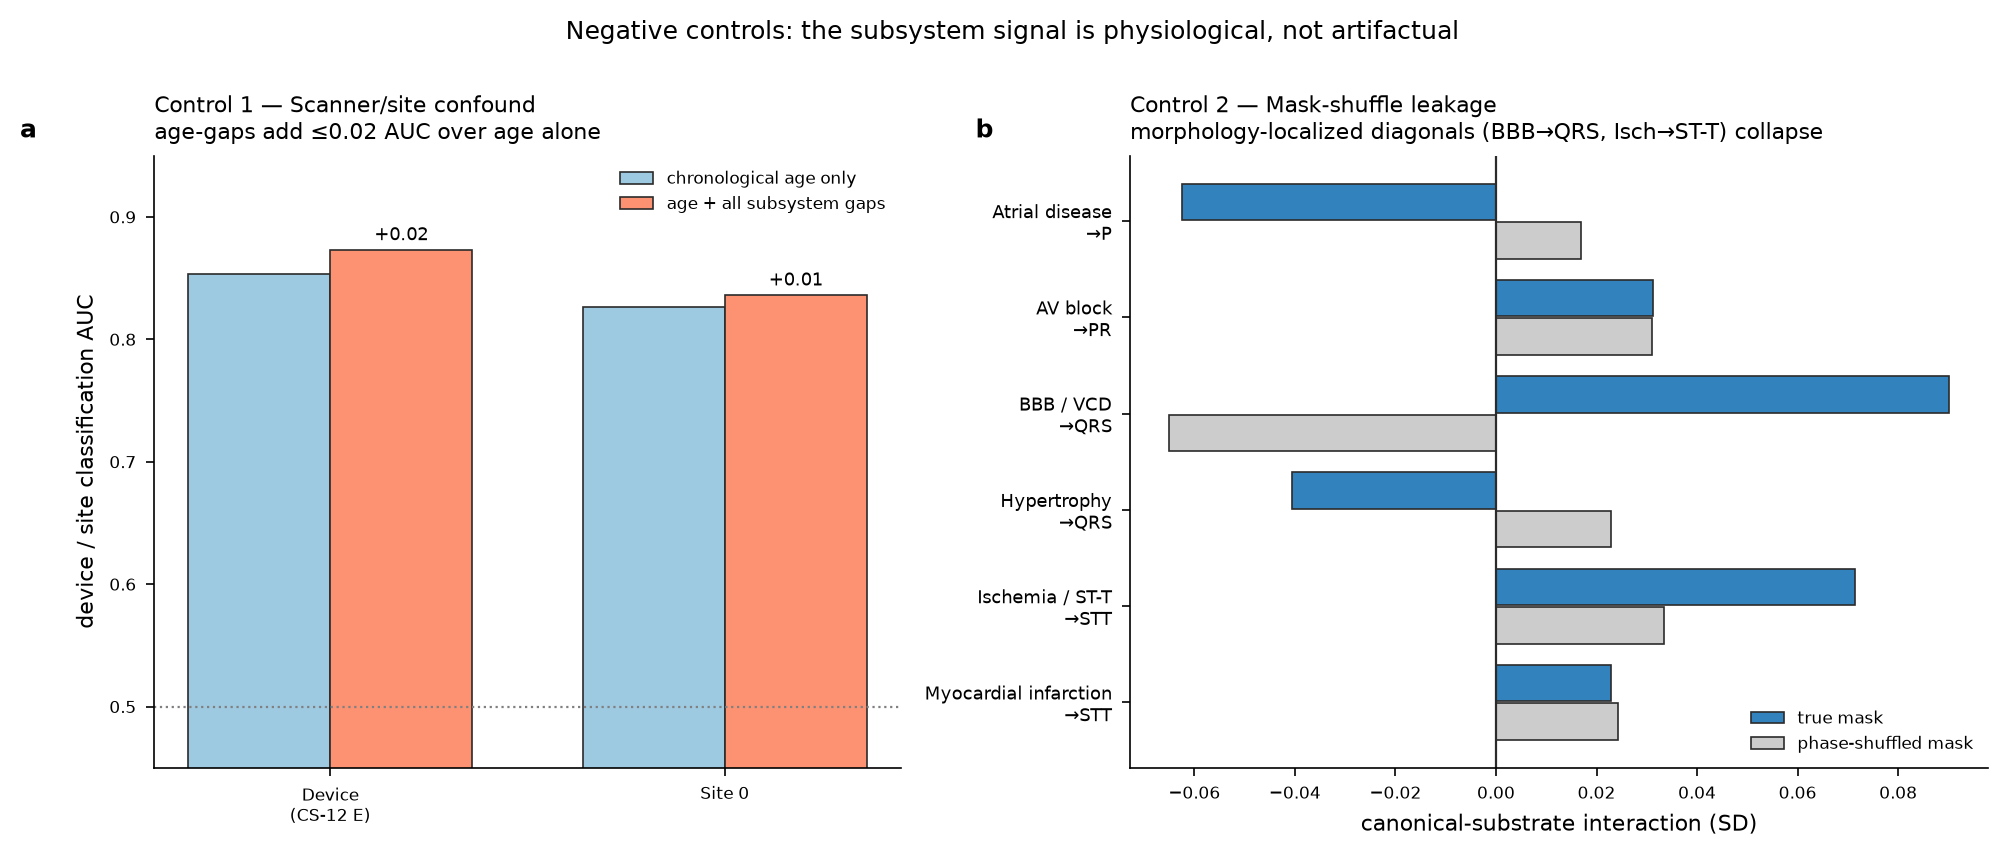
\includegraphics[width=\textwidth]{fig5_negative_controls.png}
\caption{\textbf{Negative controls.} \textbf{(a)} Subsystem age-gaps add $\le 0.02$ AUC over
chronological age when predicting recording device or site --- no covert scanner encoding.
\textbf{(b)} Under phase-shuffled masks the morphology-localized diagonals collapse relative to
the true masks, confirming the signal requires electrically-correct windowing.}
\label{fig:negctrl}
\end{figure}

\section{Results --- Act~II: the same principle predicts mortality whole-body}

\paragraph{The bridge, and what it is not.}
Act~I established, in PTB-XL, that the heart does not age as a single clock: segment-masked
electrical clocks of the atria, AV conduction, ventricular depolarization, and repolarization
diverge, and each divergence localizes to the disease that damages its substrate. That is a
claim about \emph{one organ, resolved into subsystems}. Act~II asks whether the same
organizing principle --- biological age is a profile of per-system clocks that diverge,
localize to modifiable exposure, and predict hard outcomes --- holds when we zoom out to
whole-body physiology. \textbf{NHANES and PTB-XL are different cohorts, and NHANES contains no
ECG waveforms.} Act~II is therefore \emph{not} an external validation of the Act~I electrical
clocks --- no NHANES participant contributes an ECG to any model, and no Act~I model is reused.
It is a parallel, independent demonstration that the organ-resolved-aging \emph{method}
generalizes, reproducing the Act~I signature (divergence, exposure attribution, outcome
prediction) on a second organ hierarchy in a second population, against the hardest endpoint:
all-cause mortality. The whole-body organ-age-gap construction follows established precedent
\citep{tian2023organage, oh2023organage}; our contribution is its use as the bridge, not the
idea itself.

\paragraph{Cohort.}
We pooled three continuous NHANES cycles (2005--2006, 2007--2008, 2009--2010; CDC public-use
modules) linked to the NCHS Public-Use Linked Mortality File (2019 release), giving prospective
all-cause mortality through the end of 2019. The mortality-eligible analytic sample is
\textbf{$n=\num{15844}$ adults aged 20--79 with \num{2002} deaths} over a median 11.3 years of
follow-up (\num{176489} person-years). The complete-case multi-system sample (all six clocks
present) is $n=\num{13228}$ with \num{1512} deaths.

\paragraph{Six organ-system clocks.}
For each of six physiological systems we trained an elastic-net predictor of chronological age
in disease- and medication-free participants, then took the bias-corrected age-gap (predicted
$-$ chronological, corrected against age on the healthy set) --- the Act~I construction
transposed to tabular physiology (Table~\ref{tab:organs}). Two variables were excluded from the
predictors as principled confounds, not post-hoc corrections: \textbf{total cholesterol}
(non-monotonic with age --- the ``cholesterol paradox'') and \textbf{eGFR} (computed \emph{from}
age by the CKD-EPI equation \citep{levey2009ckdepi}, which would make a renal clock partly
circular). Systems predict age with very different fidelity (healthy-cohort cross-validated
$R^2$: immune 0.03, hepatic 0.05, hematologic 0.08, renal 0.08, cardiovascular 0.10, metabolic
0.21) --- and, as below, this fidelity ordering does \emph{not} predict which clocks predict
death.

\begin{table}[t]
\centering
\caption{\textbf{Six NHANES organ-system age clocks (Act~II).} Each clock is an elastic-net
regressor of chronological age trained in healthy participants; the age-gap is bias-corrected
on the healthy set. Total cholesterol and eGFR were excluded as principled confounds.}
\label{tab:organs}
\begin{tabular}{lp{9.2cm}c}
\toprule
System & Biomarker inputs & Healthy $R^2$ \\
\midrule
Cardiovascular & Systolic/diastolic BP, pulse pressure, pulse rate & 0.10 \\
Metabolic & HbA1c, BMI, waist circumference, serum glucose & 0.21 \\
Renal & Creatinine, BUN, albumin, uric acid & 0.08 \\
Hepatic & ALT, AST, GGT, ALP, bilirubin, total protein, globulin & 0.05 \\
Immune / inflammatory & CRP, WBC, neutrophils, lymphocytes, monocyte \%, N:L ratio & 0.03 \\
Hematologic & RBC, hemoglobin, hematocrit, MCV, RDW, platelets, MPV & 0.08 \\
\bottomrule
\end{tabular}
\end{table}

\subsection{Organ-age gaps predict mortality, with a gradient across systems}

In Cox proportional-hazards models (fit with \texttt{lifelines} \citep{davidson2019lifelines})
adjusted for chronological age and sex, four of six organ-age gaps are associated
with all-cause mortality after FDR correction (Fig.~\ref{fig:cox}a, Table~\ref{tab:cox};
hazard ratios per $+1$ SD of gap). A mutually-adjusted joint model confirms the four
significant systems each retain independent signal --- they are not redundant restatements of
one frailty axis --- and the proportional-hazards assumption held for every gap (Schoenfeld
global $p>0.06$). The immune gap, null on its own (HR 1.01), takes a weak protective association
once other systems are fixed (joint HR 0.95, $p=0.004$); we read this as shared variance with
the damage-aligned systems (suppression), not as protective immune aging, and do not interpret
it as an independent effect.

Critically, \textbf{age-prediction fidelity does not explain which clocks predict death}. The
hepatic clock is one of the weakest age-trackers ($R^2\approx0.05$) yet the strongest mortality
predictor (HR 1.38); the cardiovascular clock is a moderate age-tracker ($R^2\approx0.10$) yet
carries no mortality signal --- plausibly because a cross-sectional blood-pressure age-gap is
confounded by antihypertensive treatment. The organ-age gap predicts death by capturing
pathology-relevant deviation, not by how tightly its biomarkers track chronological age.

\begin{table}[t]
\centering
\caption{\textbf{Organ-age gap and all-cause mortality (NHANES, age/sex-adjusted Cox).} Hazard
ratios per $+1$ SD of organ-age gap; $n=\num{15844}$, \num{2002} deaths. FDR by
Benjamini--Hochberg. The joint column is the mutually-adjusted six-system model.}
\label{tab:cox}
\begin{tabular}{lccc}
\toprule
System & HR (95\% CI) per $+1$ SD & FDR $p$ & Joint-model HR \\
\midrule
Hepatic        & \textbf{1.38 (1.33--1.43)} & $<10^{-60}$  & 1.30 \\
Hematologic    & \textbf{1.36 (1.33--1.40)} & $<10^{-100}$ & 1.34 \\
Metabolic      & 1.20 (1.15--1.24)          & $<10^{-20}$  & 1.21 \\
Renal          & 1.19 (1.16--1.22)          & $<10^{-8}$   & 1.12 \\
Immune         & 1.01 (0.95--1.06)          & 0.84 (n.s.)  & 0.95$^{*}$ \\
Cardiovascular & 0.97 (0.93--1.01)          & 0.19 (n.s.)  & 1.01 (n.s.) \\
\bottomrule
\end{tabular}
\end{table}

\subsection{A multi-system profile beats chronological age at predicting death}

The Act~II analogue of the added-value ladder: using leak-free out-of-fold (5-fold) Cox
predictions on the complete-case sample, Harrell's C-index \citep{harrell1996cindex} rises
monotonically (Fig.~\ref{fig:cox}b) --- age only 0.813, age$+$sex 0.817, $+$best single system
(hepatic) 0.830, $+$all six systems \textbf{0.845}. The gain of the full profile over age$+$sex
is $\Delta C = +0.028$ (95\% bootstrap CI 0.023--0.033; paired $P(\Delta C>0)=1.000$), and a
likelihood-ratio test confirms the six gaps jointly improve fit ($\chi^2_6=559$,
$p\approx2\times10^{-117}$). A person's \emph{pattern} of divergent organ clocks, not just their
age, sharpens the prediction of who dies. We independently reproduced this ladder from the
released survival table (identical values to three decimals).

\begin{figure}[t]
\centering
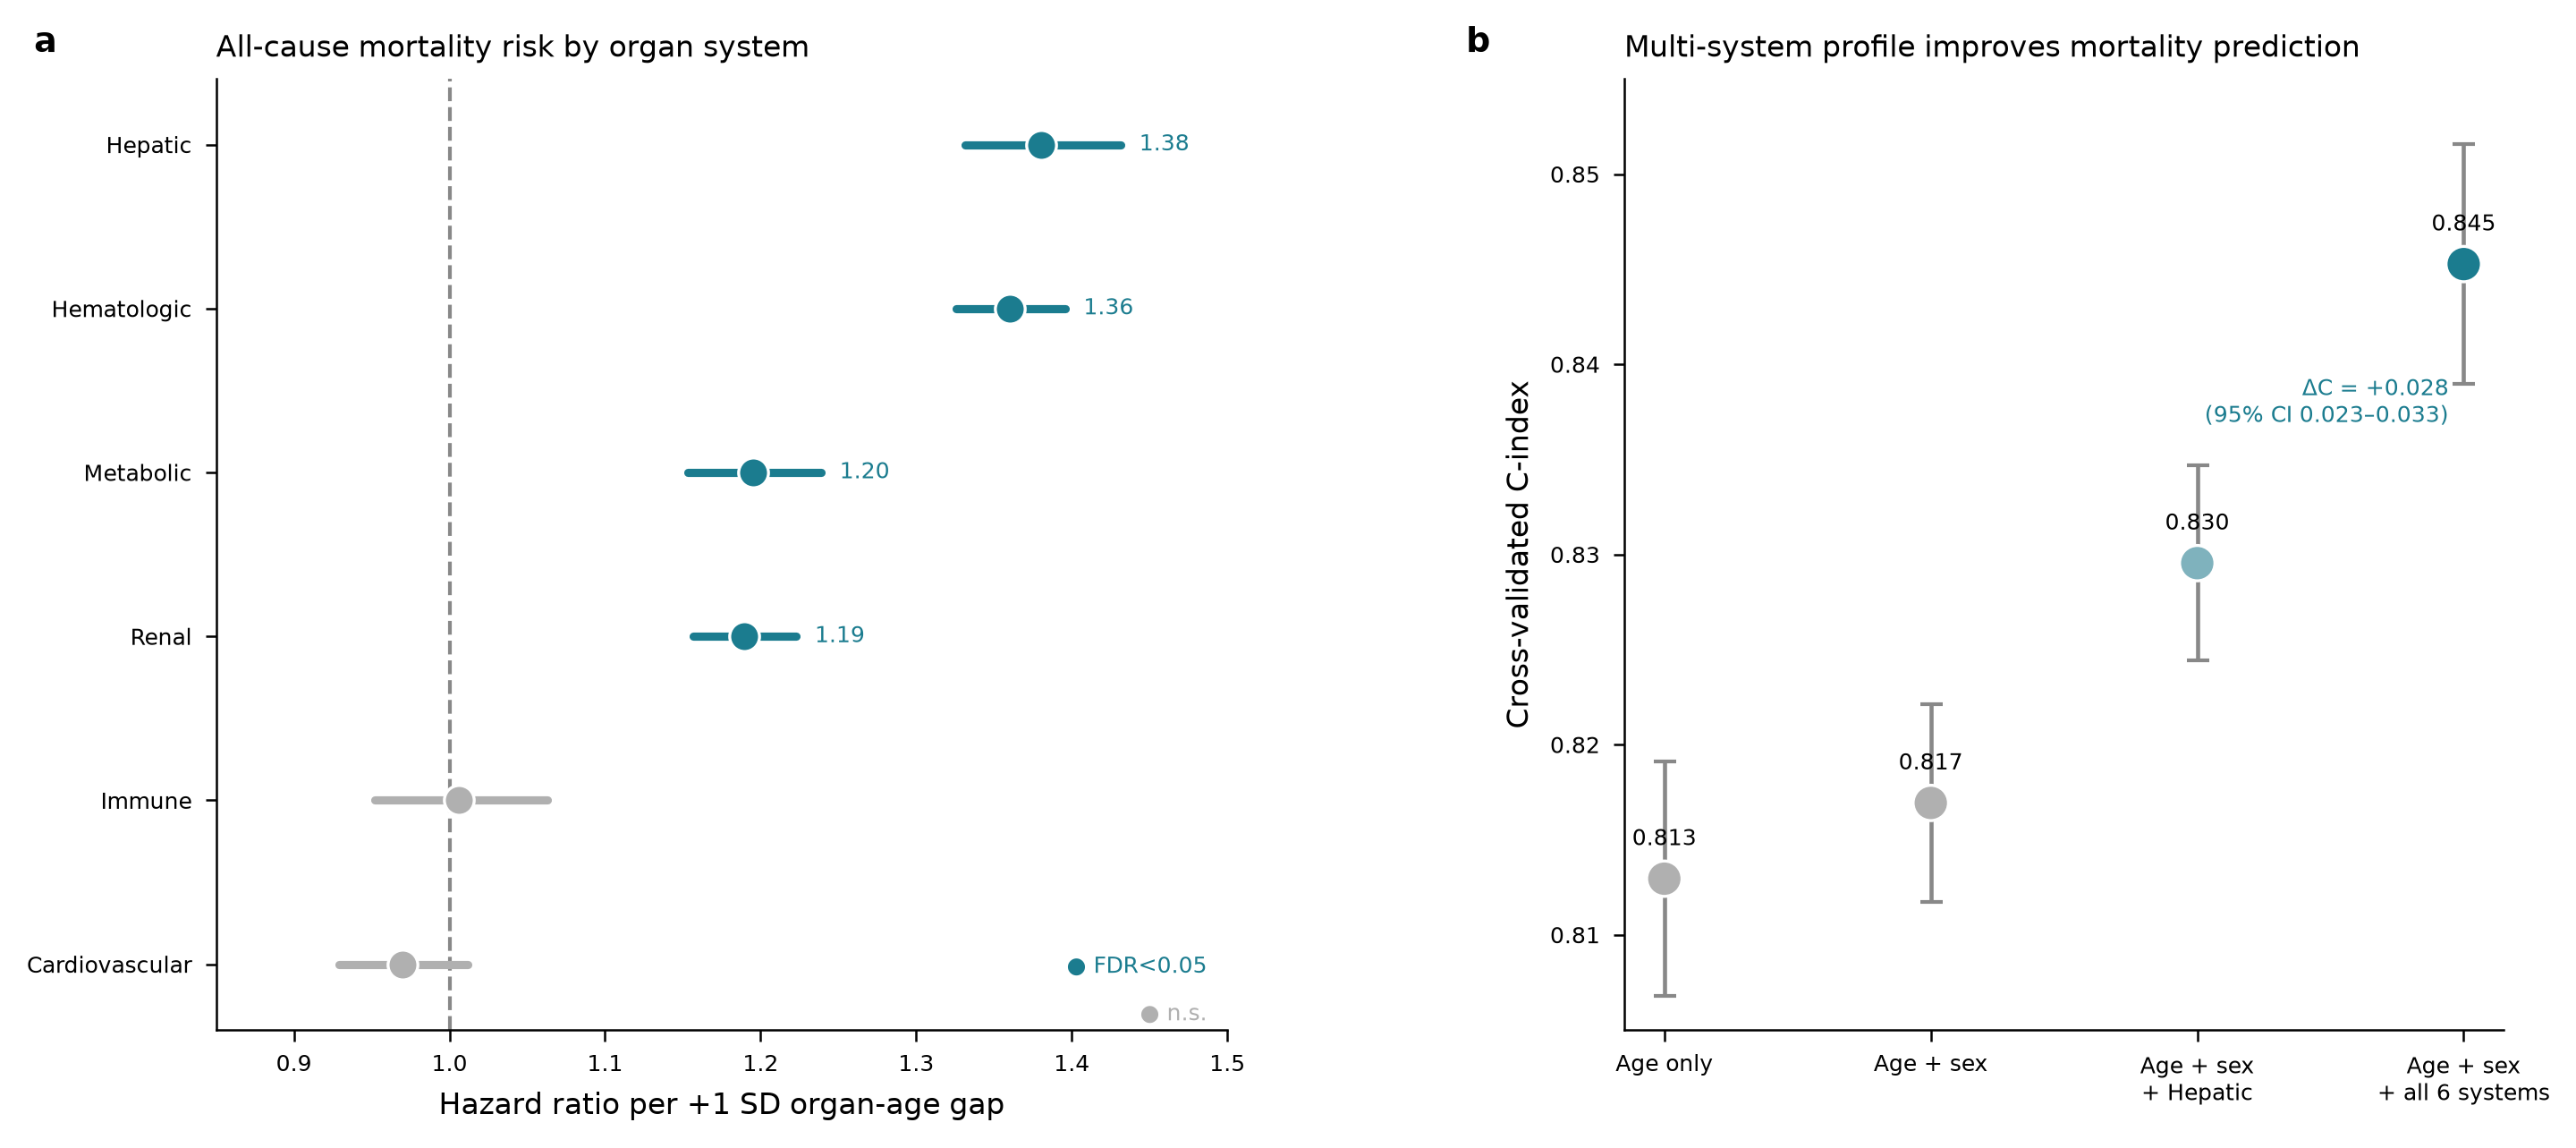
\includegraphics[width=\textwidth]{fig6_nhanes_cox.png}
\caption{\textbf{Organ-age gaps predict mortality (NHANES).} \textbf{(a)} Per-organ Cox hazard
ratios for all-cause mortality (per $+1$ SD organ-age gap, adjusted for age and sex;
$n=\num{15844}$, \num{2002} deaths). Teal = FDR-significant, grey = not significant.
\textbf{(b)} Out-of-fold cross-validated C-index for nested models; the six-system profile adds
$\Delta C=+0.028$ (95\% CI 0.023--0.033) over age$+$sex.}
\label{fig:cox}
\end{figure}

\subsection{A modifiable exposure ages the same clocks that predict death}

Act~II's localization test uses a modifiable exposure: smoking. Comparing never/former/current
smokers (Fig.~\ref{fig:smoking}), the two systems with the largest mortality hazard ratios ---
hepatic and hematologic --- are exactly the two with the cleanest monotonic dose-response: the
hematologic clock runs 2.1 years older and the hepatic clock 1.1 years older in current versus
never smokers (both FDR $p<10^{-50}$), stepping up cleanly through former smokers. The two
systems that carry no mortality signal (immune, cardiovascular) show no coherent monotonic
smoking gradient. This is the same closing move as Act~I --- the divergence points at its cause
--- now with an exposure a person can change.

\begin{figure}[t]
\centering
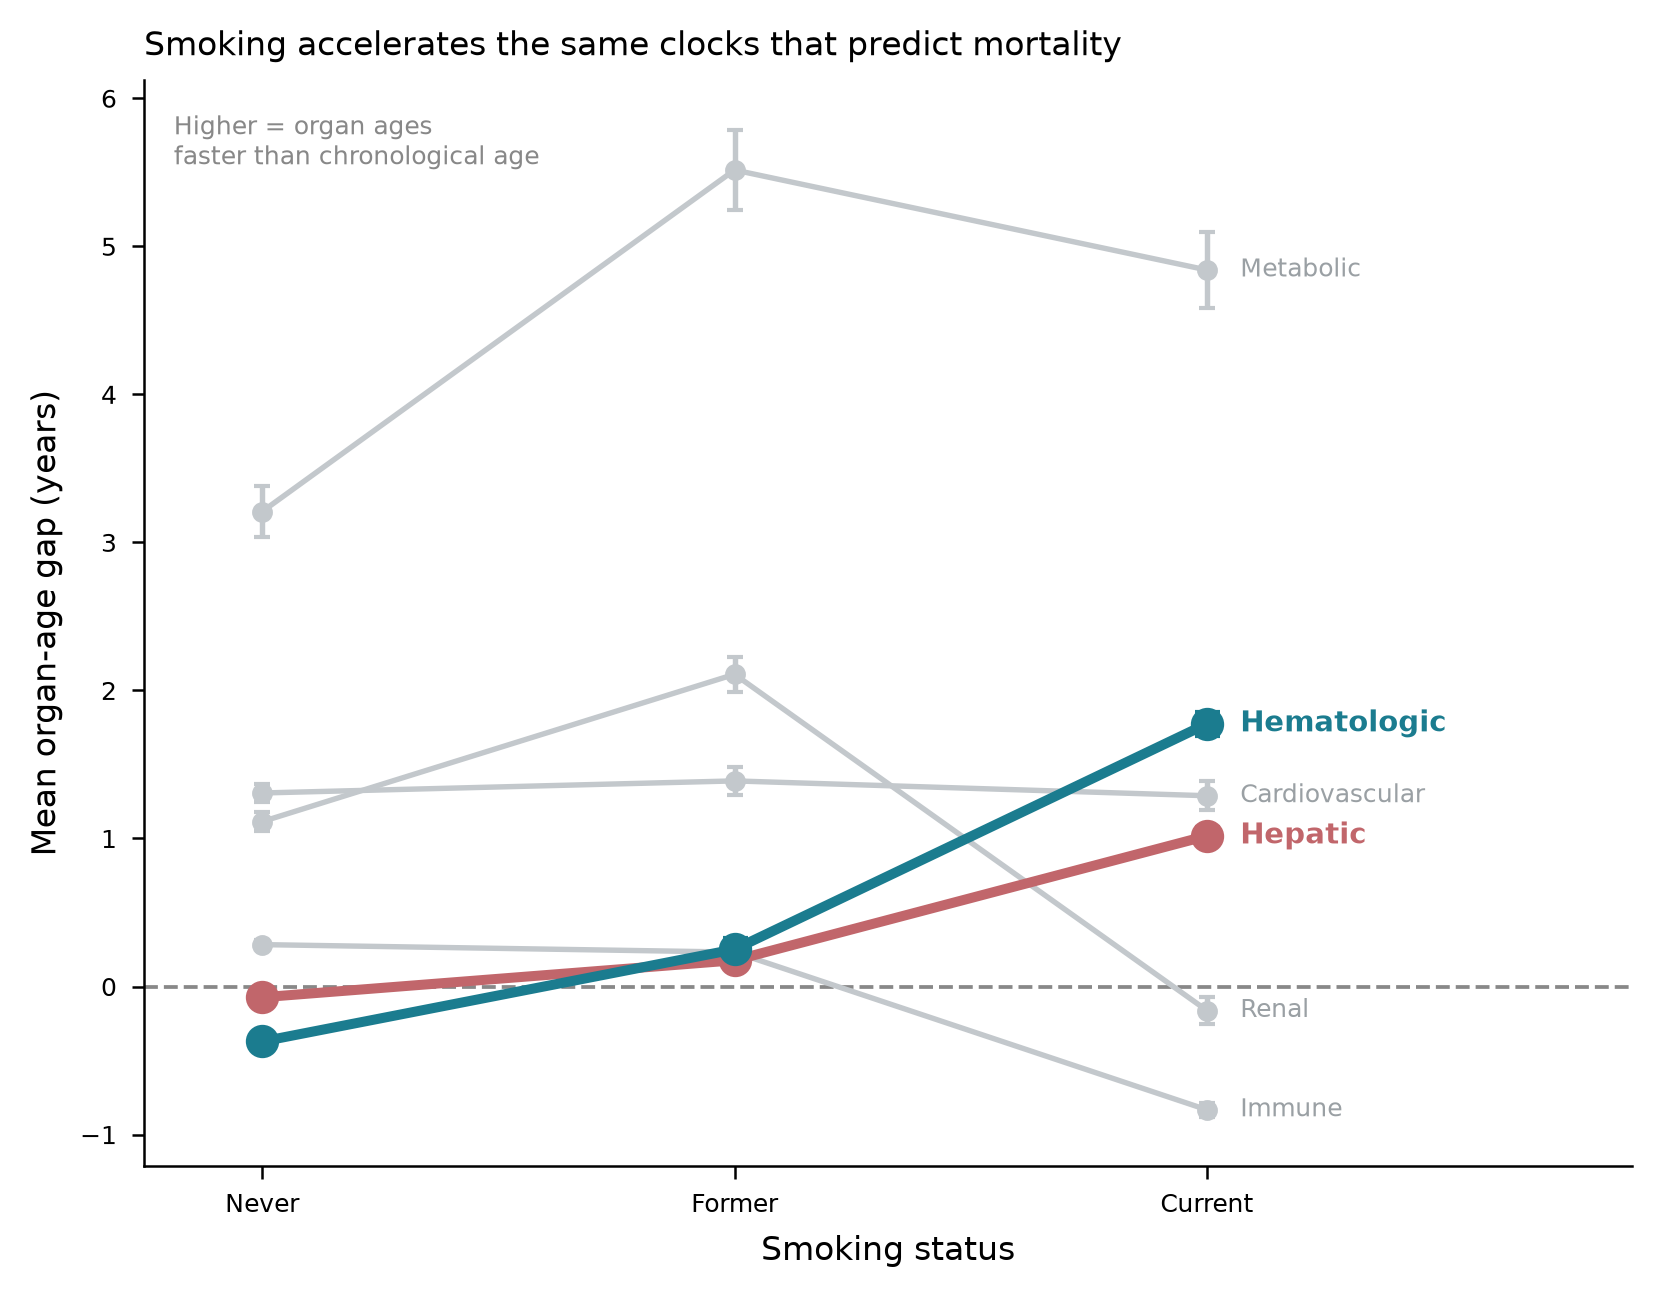
\includegraphics[width=0.72\textwidth]{fig7_nhanes_smoking.png}
\caption{\textbf{Smoking accelerates the same clocks that predict mortality.} Mean organ-age gap
by smoking status. The two systems with the highest mortality HRs (hepatic, hematologic, in
color) show the cleanest monotonic acceleration with smoking; weak/null systems (grey) do not.}
\label{fig:smoking}
\end{figure}

\section{Discussion}

Subsystem-resolved ECG aging converts a single opaque ``ECG age'' into a four-dimensional
electrical-age fingerprint whose shape is clinically interpretable. The fingerprint recovers
the canonical substrate for single-substrate conduction and repolarization diseases and reveals
physiologically-real cross-substrate aging for multi-system diseases --- behavior consistent
with cardiac electrophysiology, stable across two independent pipelines, and supported by
patient-cluster bootstrap confidence intervals and two negative controls. Act~II shows the same
organizing principle is not specific to the heart's electrical anatomy: transposed to whole-body
physiology in an independent national cohort, per-organ age-gaps diverge, localize to a
modifiable exposure (smoking), and predict all-cause mortality beyond chronological age. The
method --- train per-system age predictors in healthy people, read out the bias-corrected
age-gap, ask what it localizes to and what it predicts --- is the contribution, and it
reproduces across two measurement modalities and two populations. The pattern echoes the
whole-body organ-aging literature \citep{tian2023organage, oh2023organage} while extending it
downward, into the electrical subsystems of a single organ.

A design theme runs through both acts: the informative signal appears only after the obvious
confounds are removed. The raw ``which subsystem is oldest'' readout localizes in only 2 of 6
diseases; the double-centered interaction and within-patient contrast recover the substrate
map. Whole-body clocks required excluding total cholesterol and eGFR before their age-gaps were
interpretable. And the mortality analysis deliberately avoids a single mutually-adjusted model
of causally-sequential exposures, which risks the Table~2 fallacy \citep{westreich2013table2}.
Throughout, age-gaps are bias-corrected in the manner established for brain-age
\citep{beheshti2019biascorr, delange2020biascorr, zhang2023residualbias}.

\paragraph{Limitations.}
PTB-XL is a single-institution cross-sectional cohort; the ECG age-gaps are not linked to
prospective outcomes within PTB-XL here (the NHANES analysis, on a disjoint population with no
ECG waveforms, is a parallel demonstration of the method, not external validation of the ECG
clocks). The substrate-pure analysis (\S\ref{sec:pure}) is power-limited for the rarer groups.
Subsystem accuracy is bounded by delineation quality, particularly for the short PR segment and
the J-point-sensitive ST--T boundary. The atrial clock's paradoxical behavior in atrial
fibrillation --- where its own input signal is destroyed by the disease --- is a fundamental,
not incidental, limitation of P-wave-based atrial aging. The NHANES analysis is complete-case
and unweighted, so its estimates are associational rather than nationally representative, and
its organ clocks are built from routine labs rather than the plasma-proteomic or imaging panels
used elsewhere \citep{tian2023organage, oh2023organage}.

\section*{Data availability}
\addcontentsline{toc}{section}{Data availability}
This study uses only openly-available data. PTB-XL v1.0.3 is distributed through PhysioNet
\citep{wagner2020ptbxl, goldberger2000physionet}
(\url{https://physionet.org/content/ptb-xl/}). NHANES 2005--2010 public-use modules are
distributed by the CDC (\url{https://wwwn.cdc.gov/nchs/nhanes/}) and linked to the NCHS
Public-Use Linked Mortality File, 2019 release
(\url{https://www.cdc.gov/nchs/data-linkage/mortality-public.htm}). No participant-level data
are redistributed with this work; the accompanying repository ships download and preprocessing
scripts only, in accordance with the PhysioNet and NCHS data-use agreements.

\section*{Code availability}
\addcontentsline{toc}{section}{Code availability}
All extraction, training, and analysis code; the trained subsystem clocks; the per-ECG and
per-participant prediction tables; and the specificity, negative-control, and mortality analyses
are provided in the accompanying repository, together with a scripted pipeline to reproduce
every figure and table from the released prediction tables.

\section*{Ethics}
This work is a secondary analysis of two de-identified, publicly-available datasets released
under their respective data-use agreements (PhysioNet Credentialed Health Data Use Agreement for
PTB-XL; NCHS public-use and linked-mortality terms for NHANES). No new data were collected and
no identifiable participant information was accessed; the analysis is therefore not human-subjects
research requiring additional institutional review.

\section*{Author contributions}
J.M.\ conceived the study, designed and implemented the analyses, and wrote the manuscript.

\section*{Competing interests}
The author declares no competing interests.

\section*{Funding}
This research received no specific grant from any funding agency in the public, commercial, or
not-for-profit sectors.

\section*{Use of AI tools}
The analyses and manuscript were developed with the assistance of an AI research agent used for
code implementation, statistical analysis, figure generation, and drafting under the author's
direction. The author verified all results, reproduced the primary mortality analysis
independently, and takes full responsibility for the content.

\bibliographystyle{unsrtnat}
\bibliography{references}

\end{document}
